\parindent=0em
\subsection{HMD Odyssey+}
\label{sec:odyssey}
\noindent

%https://www.samsung.com/hk_en/news/product/reality-headset-hmd-odyssey-plus/

El casco \textit{HDM Odyssey+} (figura~\ref{fig:hdmOdysseyVista}) es un dispositivo desarrollado por la empresa \textit{Samsung} que salió al mercado en 2018, no es un casco independiente ya que requiere estar conectado a un ordenador compatible con la plataforma \textit{Windows Mixed Reality} para funcionar, se conecta al ordenador mediante un cable \textit{HDMI}~2.0 y un \textit{USB}~3.0.

\begin{figure}[h]
    \centering
    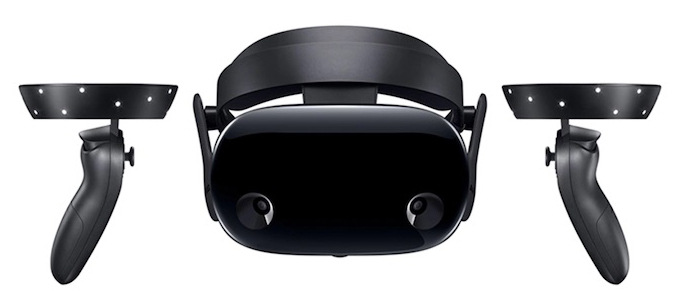
\includegraphics[scale=0.6]{Images/Estado del arte/samsungOdysseyplus.jpg}
    \caption{HDM Odyssey+ dispositivo al completo.}
    \label{fig:hdmOdysseyVista}
\end{figure}

En cuanto a la parte de monitorización de la imagen, este casco tiene una resolución de 1.440 x 1.600 píxeles por ojo, un total de 2.880 x 1.600 píxeles combinando los dos ojos, además, el \textit{Field of View} abarca un total de 110º. Este dispositivo no posee tecnología de \textit{hand tracking} (por lo que controla el movimiento de manos con dos mandos que funcionan con pilas) y tampoco tiene \textit{eye tracking}, en cambio, destaca por tener dos sensores \textit{6DoF} frente al único que tiene, por ejemplo, las \textit{Hololens~2} (sección~\ref{HoloLens2Dispositivo}).\\

Por otra parte, está dotado de sensores como acelerómetro, giroscopio, brújula y sensor de proximidad (este último se utiliza para saber en qué momento se lleva puesto el casco), del mismo modo, posee una diadema que se puede  modificar para ajustar el casco a la cabeza de cada individuo, sin embargo, este dispositivo no está diseñado para ser utilizado con gafas.\\ 

Por último, tiene un sensor que ajusta automáticamente la \textit{IPD}, conexión \textit{bluetooth} y un peso total de 644g teniendo en cuenta solo el \textit{HMD} y un añadido de 176g si se cuenta el peso del cable.


\footnotetext[1]{
\label{hdmOdysseyfooter}{Imagen de la HDMOdyssey+: \url{https://www.samsung.com/us/computing/hmd/windows-mixed-reality/hmd-odyssey-windows-mixed-reality-headset-xe800zba-hc1us/}.}}

\footnotetext[1]{
\label{hdmOdysseyfooter}{Especificaciones de la HDMOdyssey+: \url{https://www.microsoft.com/en-us/p/samsung-hmd-odyssey/8n2d0nk20p8m?cid=msft_web_collection&activetab=pivot:techspecstab}.}}